\documentclass[a4paper,12pt]{article}

\usepackage{amsmath,amssymb}
\usepackage[dvips]{graphics}

\DeclareMathOperator{\dd}{d}

\newcommand{\prm}{\partial_{\mu}}
\newcommand{\prn}{\partial_{\nu}}
\newcommand{\prj}{\partial_{j}}
\newcommand{\prk}{\partial_{k}}

\begin{document}

	Dynamical models with compact-valued variables receive more 
	and more attention in the modern physics.
	A valuable example of such models is the construction
	proposed by L.~Faddeev more than 25 years ago
%        The so-called Faddeev-Skyrme model, first introduced in the
%        work 
\cite{LF}.
%       in the present time draw more and more attention in different areas
%        of science.
        This model has nontrivial applications in the condensed matter 
        physics
\cite{},
        physics of plasma, its extension emerges in the description
        of the infrared limit of the 
    $ SU(2) $
        Yang-Mills theory
\cite{}.

        One of the main properties of the Faddeev-Skyrme model is the
        possibility to represent its statical solutions as knots 
        composed of closed twisted vortex tubes.
        At the same time, as was shown in
\cite{VK}
        the energy of a solution admits a nontrivial
        lower bound estimate in terms of its topological characteristic
        --- Hopf charge. This charge can be represented via
        the linking number of the vortex tubes.

        This work describes in a very speculative way 
        the connection between the concept of the vortex tubes and the
        the VK estimate in the region of high energies. 
        It allows authors to make an assumption about the 
        area of applicability of the fit derived from VK estimate. 
        We provide two constructive examples of sequences of
	knotted configurations which stay
????        in tact with the VK estimate.
%	The main faraway goal of this investigation is to shed some
%	light on the form and view of the Faddeev-Skyrme solitons
%	with the high energies.
	We argue that the proposed concept of the vortex
	tubes along with the VK estimate is a powerful tool in
	analyzing high energy static configurations of the
	Faddeev-Skyrme model.

        Let us discuss this model in more detail.
        Its lagrangian is the following Lorentz-invariant expression
        over a compact-valued field 
    $ \vec{n} $
\begin{equation}
    L = g (\prm \vec{n})^{2} + (\prm \vec{n} \times \prn \vec{n})^{2} ,
\end{equation}
        where 
    $ \vec{n} $ 
        takes values in a two-dimensional sphere 
    $ S^{2} $.
        This lagrangian includes a single dimensional constant 
    $ g : [g] = (\text{Length})^{-2}$.

        One can associate with an arbitrary function 
    $ \vec{n} $ 
        a  3-form
\begin{equation}
    J = F \wedge A ,
\end{equation}
        where
\begin{gather}
    F = (\prm \vec{n} \times \prn \vec{n} , \vec{n}) \dd x_{\mu} 
        \wedge \dd x_{\nu}
\\
    \dd A = F .
\end{gather}
        The forms 
    $ F $ and 
    $ J $
        are closed as long as the length of the vector
    $ \vec{n} $ 
        is fixed 
    ($ \vec{n} $ 
        is expressed via two Euler angles).
        Due to this fact, the integral of the form
    $ J $
	over the spatial coordinates
\begin{equation}
\label{HC}
    Q = \int_{R^{3}} F \wedge A
\end{equation}
        is a conserved quantity.

        At the same time, if we compactify the model by fixing
        the limit 
%    of
%    $ \vec{n} $
        at infinity to some vector
    $ \vec{n}_{\infty} $,
        then
    $ \vec{n} $ 
        describes (at a fixed time) a map
\begin{equation}
    S^{3} \to S^{2} ,
\end{equation}
        and 
    $ Q $
        becomes an integer topological characteristic of this map ---
        the Hopf charge.

        Static solutions of the model are obtained by minimizing
        the potential term of the lagrangian:
\begin{equation}
    E = g (\prk \vec{n})^{2} + (\prk \vec{n} \times \prj \vec{n})^{2} .
\end{equation}
        By applying the general expression for the Hopf charge 
(\ref{HC})
        to the particular potential term 
    $ E $
        it is possible to derive the Vakulenko-Kapitansky inequality
        (VK estimate)
\begin{equation}
\label{VK}
    E \ge \text{const} \, Q^{3/4}.
\end{equation}
        An immediate and a very important consequence of this inequality
        is that a superposition of two static solutions separated
        in the space, in general, is not again a configuration
        with minimal energy, i.~e. there is a nontrivial interaction.

\section{Conception of the Vortex Tubes}
        Static solutions of the Faddeev-Skyrme model have a very 
        intuitive description in terms of vortex tubes.
        In what follows we assume that the limit of the vector 
    $ \vec{n} $
        at infinity is the North Pole of the sphere 
    $ S^{2} $
        or, in components, the vector 
    $ (0,0,1) $.
        Then the preimage of the South Pole is a closed and, in general,
        multiply-connected curve. This curve is a core of a knot.
        Preimage of a vicinity of the South Pole is, in turn, a set
        of the closed curves which make up a tube. In a common case
        a contour around the core of the soliton
        is mapped to a contour around the South Pole with a nontrivial index.
        But experiments 
\cite{}
        show that it is not the case for static
        configurations.

        From topology we know that the Hopf charge 
    $ Q $
        of the map 
    $ \vec{n} $
        is the link number of the curves --- preimages of two arbitrary
        distinct points in the target. It is our choice to choose for that
        purpose the core line and preimage of any other point in the vicinity
        of the South Pole.
        Simple considerations show, that in stable configurations the
        lines that constitute the tube wrap around the core, that is the
        tube is twisted (this is obvious for toroidal configurations,
	they should be twisted in order to be stable).

        The concept of the vortex tubes thus implies that static
        configurations  possess several characteristic parameters
        which depend only on the 

?????constant of interaction ?????
	coupling constant

    $ g $
        of the model, but not on the energy and Hopf charge (i.~e. they
        are local parameters). Among them are the optimal number of twists
        per unit length 
    $ \Lambda $
        and the linear density of energy 
    $ \rho $
\cite{NS}.

        In order to consider static solutions of the model as knotted
        vortex tubes it is necessary to introduce one more parameter,
        namely, the radius of the tube, or half of the typical 
        distance in between the cores of the adjacent tubes.
        In any particular point this distance depends on the angle
        between the cores, on their longitudinal bend, as well as on
        their twist (which is a local parameter). But nevertheless we 
	shall assume that at least some average radius
    $ r $
        enters the model as a local character.

        Existence of such a radius is a nontrivial fact.
        Moreover, simple calculation shows, that for instance two parallel
        twisted tubes tends to attract, there is no stable distance of
        interaction in this configuration.
        We intend to justify the notion of the radius of vortex tubes
        in the oncoming article.

        Thus the model in question contains three character
        dimensional parameters, which are defined by a single coupling
        constant 
    $ g $.
        We can express this fact by the following relation
\begin{equation}
    g = \Lambda^{2} = r^{-2} = \rho ,
\end{equation}
        which we expect to hold at least up to some dimensionless factors.

        And finally we would like to supplement the concept of the vortex
        tubes with a simple ``selection rule''. It says that the images of
        two contacting points of the adjacent tubes in the knot should be
        mapped into the same point on the target sphere.
        Being a trivial consequence of the continuity of the map 
    $ \vec{n} $,
        this rule allows to explain less trivial things, like the magical
        charge 7 of the trefoil configurations
\cite{}.
	We won't employ this rule in the present paper and leave it as a tool
	for finer calculations.

\section{Relation??ship?? between vortex tubes and the VK bound}
        In this part we shall provide a speculative relationship
        between concept of the vortex tubes and the Vakulenko-Kapitansky
        estimate. 
        More precisely, we are going to show, that in big
        enough static configurations the topological charge 
    $ Q $
        is proportional to the energy to the power 
    $ 4/3 $:
\begin{equation}
\label{QE}
    Q \sim E^{4/3} .
\end{equation}

	The calculation is the following. According to the conception
	described above, we consider
	our soliton as a thin elastic tube, of a constant radius
    $ r $
	(or a constant area $ s $),
	whose energy is proportional to its length
    $ L $ (to the leading order).
	The tube is bundled in a knot and its ends are clamped.
	Of course, the knot may be multiply-connected - i.~e. the solution
	may consist of several rods. 
	With these assumptions the linear size 
    $ x $
	of the knot is proportional to the volume (and to the length
    $ L $)
	to the power of one third
$$ x \sim L^{1/3} . $$
%	The Hopf invariant of the soliton
%	is the sum of the number of twists and its (self)linking number:
%   $$ H = H_{twist} + H_{link} .$$
%	The first one is proportional\footnote{We may not increase 
%the number of twists per unit lenght, since
%from some point the energy depends quadratically on it \cite{MNS}.}
%	to the length $ L $, that is to the 
%	energy $ E $, which spoils the picture for the small energies,
%	but could be neglected as the energy grows.
	In order to calculate the Hopf invariant
	we should pull apart the preimages of the south 
	pole and of a point in its vicinity while 
	counting the number of ``unlinking operations'' between them.
	For a tight knot the number of unlinking operation needed
	to withdraw a piece of core of unit length is proportional to the
	linear size of the knot 
    $ x $. 
	This is because, for a dense knot,
	a piece of core of a length
    $ 2r $
	needs roughly one unlinking operation in order to be moved to
	the distance
    $ 2r $ and
    $ \frac{x}{2r} $
	operations to be moved to the distance
    $ x $.
	Hence the whole number of unlinking operations is proportional to
\begin{equation}
\label{HH}
	Q \sim L x \sim L^{4/3} \sim E^{4/3} .
\end{equation}

	Being very simple and speculative, the presented calculation
	however, reveals the nature of the nontrivial ``three-fourth'' power
	in the VK estimate. This power stems from self-linking 
	and from linking of the connected components with
	each other, twisting could be neglected with respect to them.
	We can clearly see from above that ``three-fourth'' is 
	applicable only when the size of the knot is sufficiently
	large with respect to the radius of the tube, or in other
	words when the energy and the Hopf invariant are high enough.
	There is no indication that ``three-fourth'' behavior is correct
	for small charges.
	Original constant ?? in the RHS of
(\ref{VK})
	was received in a precise mathematical derivation and it
	serves in all range of energies/charges.
	The numerous attempts to reduce this constant 
	that are present in the modern literature should be done first for 
	high energies.

%	We may notice here, that the contribution of twist of the tube,
%	according to our conception, is proportional to to the length
%	of the tube, that is to the energy of the soliton.
%	This means that for high enough energies twisting does not 
%	play the role in the VK estimate.

\section{Trivial consequence}
	Simple calculation which we have presented above allows
	to estimate the average length of the connected components
	of the knot. First we may propose that this length 
    $ l $
	is a function of the linear size of the knot:
\begin{align}
    l & = l(x), \\
    L & = k l(x) ,
\end{align}
	where 
    $ k $
	is the number of connected components.
	The upper bound of 
    $ l $ 
	is the full length 
    $ L $
	which is defined by the energy of the configuration.
%	First estimate for the lower bound is a constant.
	We can roughly estimate the upper limit of the linking
	number of each connected component with the rest components
	of the knot by the following expression:
\begin{equation}
    4 \pi (\frac{l(x)}{2 \pi})^{2} \cdot \frac{1}{4 \pi r^{2}} =
	(\frac{l(x)}{2 \pi r})^{2} \sim l^{2}(x) ,
\end{equation}
	where 
    $ 4 \pi (\frac{l(x)}{2 \pi})^{2} $
	is the square of the circle for which 
    $ l(x) $
	is the length of the boundary.
%	and 
%    $ 4 \pi r^{2} $
%	is the square of the section of the tube.
	Thus the Hopf invariant of the knot can be estimated simply by
	multiplying this quantity by 
    $ k $
	and adding the contribution of self-linking of the
	connected components:
\begin{equation}
    Q \lesssim k l^{2}(x) + k l^{4/3}(x) \sim k l^{2}(x) \sim L \cdot l(x) .
\end{equation}
	On the other hand
    $ Q $
	has the order of 
    $ L \cdot x $
	and thus
\begin{equation}
\label{bnd}
    x \lesssim l(x) \lesssim L \sim x^{3} .
\end{equation}
	As we shall argue later this estimate could not be improved
	in the frames of 
????
VT conception. We shall present candidates

	for static configurations with lengths of the connected
	components varying in the boundaries of the inequality
(\ref{bnd}).
	This estimate also yields that no high energy solution
	could be constructed from fixed length (energy) knots without
	reconnecting them in the bigger connected components.

\section{Two examples}
	Now that we have provided some arguments in favor
	of conception of the vortex tubes and its consistency
	with VK estimate, it is the time to present constructive
	examples. Each example is a sequence of configurations
%	composed from vortex tubes, 
	with the energy and the Hopf charge increasing according to
(\ref{QE}).
	We propose these configurations as candidates for
	initial points for numerical experiments in the high
	energy region.
	A very degenerate case of the proposed examples is the
    $ H=8 $
	soliton from the work
\cite{BS}.
	
	Both sequences represent stretched linear objects composed of
	elementary tubes intertwined in some way. Center lines
	of these objects may constitute any simple closed curve(s)
	like unknot, trefoil, linked rings, etc.
	The difference between the examples is only in the way of
	intertwining the tubes.

	The first example looks as follows.
	It is built of cylindric layers successively put one
	upon another. Each layer is spanned with elementary tubes
	wrapping the previous layer at a definite small angle
	to the center line. The ends of the whole structure
	are clamped in such a way that elementary tubes at each end
	are connected with the tubes of the same layer.

	Let us estimate the energy and the Hopf charge of this configuration.
	For simplicity we shall count the number of layers (and the
	number of configuration in the sequence) using the radius of the tube
    $ R $.
	It is natural to assume that, in order for the construction
	to be knotted in a ring, trefoil, etc, its length 
    $ L_{\text{l.c.}} $
	should be proportional to 
    $ R $.
	That is, its energy is proportional to 
    $ R^{3} $.

	Since the angle between the center line and the elementary
	tube is a fixed small value, their linking number is proportional
	to the length of the construction (that is to 
    $ R $)
	and inversely proportional to the number of the 

????layer/layers.
	An elementary tube here, depending on the way of clamping the
	layers, means the part of the tube that goes once along
	the center line.
	The linking number of all tubes in the layer and the center line
	is proportional just to 
    $ R $,
	and that of all the tubes in all layers and the center line
	is proportional to 
    $ R^{2} $.
	Now we may notice that in this construction the linking number
	of each two elementary tubes is equal to the smallest of their
	linking numbers with center the line.
	This readily shows that the overall linking number of the
	configuration is proportional to 
    $ R^{4} $.
	A more accurate derivation gives the result
\begin{equation}
    Q = \frac{1}{3} \pi^{2} L_{\text{l.c.}} \tau r^{-4} R^{3},
\end{equation}
	where 
    $ \tau $
	is the tangent of the angle between a tube and the center line.
% and
%    $ n $
%	is the number of layers in the configuration.

	The length of each connected component in this example depends
	on the order in which the tubes are 

connected in???? connected into, joined into
the layers.
	It may vary from 
    $ R $ 
	in the center to 
    $ R^{2} $
	in the top layer if it is 
????spanned /consists of?

by one component.

	The second example is well known as a rope.
        Let us twist two or three elementary tubes, by wrapping 
        them around each other in a rope of higher order. 
	Several such ropes can be twisted 
        in the next order rope and so on --- in the end we have a thick rope
        of the order 
    $ n $. 
	Then we can glue elementary tubes at the ends 
        of the rope in such a way that it forms an unknot or other construction
	like in the previous example.
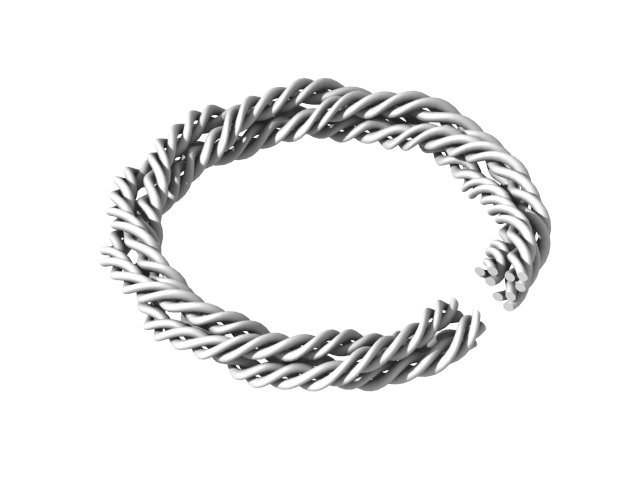
\includegraphics[40,40]{x1.gif}
        One may roughly estimate the linking number of this rope in
        the following way.
        The number of ropes $ b $, which form the rope of the next order 
        is the ``base'' of the construction. 
	There is the following relation for the radius of the rope of the
        order $ k$:
$$ \pi R^{2}_{k} \simeq \pi b^{k-1} r^{2} ,$$
$$ R_{k} \sim b^{k/2} .$$
        The linking number of two adjacent ropes of the order $ k$ 
        is proportional to their length divided by the radius 
        of the braid:
$$ h_{k} \sim \frac{x}{R_{k}} .$$
        (We assume that the tubes in the rope are crossed at fixed small angle
        in each order.) 
%	(then the shortening of the wires from order
%        to order after twisiting is just a correction to the base number 
%    $b$.)
        Hence the linking number of an elementary tube from a rope of the
        order $ k$ with all the tubes in $ b-1 $ ropes
        of the order $ k $ adjacent to the rope under consideration is 
    $ h_{k} (b-1) b^{k-1} $. 
	The linking number of an elementary
        tube with all other tubes is the sum for all orders:
$$ h = \sum^{n}_{k=1} h_{k} (b-1) b^{k-1} \sim
        \sum^{n}_{k=1} (b-1) \frac{x}{b^{k/2}} b^{k-1}
        = x \frac{ (b-1) (b^{n/2+1/2} -1)}{b(b^{1/2} -1)} \sim x b^{n/2}. $$
        The overall number of elementary tubes in a rope is
$$ b^{n-1} \sim x^{2}, $$
        and we can see that
$$ H_{link} = b^{n-1} h \sim x^{4} \sim E^{4/3} .$$

	The above calculation does not consider the shortening
	of the ropes from order to order. When we account for it,
	the rope configuration turns out to satisfy
\begin{equation}
    E^{4/3}_{n} / H_{n} \sim (1 + \alpha)^{n} ,
\end{equation}
	where 
    $ \alpha $
	is a small quantity which depends on the angle between the tubes.
	This relation implies that the sequence under consideration 
	may not bring the minimum to the energy functional.
	However, in exact experiments some other effects may come
	to the play, like the dependence of
    $ r $
	on the angle between the tubes.
	One of the arguments in favor of the rope configurations
	is that the previously mentioned ``selection rule'' holds here at every
	step for every order.

	The rope configurations are also an instructive example on the
	inequality 
(\ref{bnd}).
	When clamping the ends of the construction we can shift
	the ropes in each order in such a way that the lengths
	of the connected components will vary from
    $ x $
	to 
    $ x^{3} $ 
	(In the last case the configuration consists of only
	one connected component).

\end{document}
